\documentclass[a4paper,12pt]{report}

\usepackage{alltt, fancyvrb, url}
\usepackage{graphicx}
\usepackage[utf8]{inputenc}
\usepackage{float}
\usepackage{hyperref}

\hypersetup{
    colorlinks=true,
    linkcolor=black,
    filecolor=magenta,      
    urlcolor=blue,
    pdfpagemode=FullScreen,
    }

\title{Assignment 02 - \\``Smart Waste Disposal System''\\
    \large ``Embedded Systems e Internet of Things'' final report}

\author{Lorenzo Cinelli}
\date{\today}

\begin{document}

\maketitle

\tableofcontents

\chapter{Analysis}

    \section{Description}

        The system required is a smart waste disposal system for - potentially dangerous - liquids. It has to be composed by a container having some sensors to check the temperature of the waste and the filling level. It has also two leds and a screen to signal if the user can spill the waste or not in case of some behavior. To spill the waste there is a door controlled by two buttons - one to open it and one to close it. 
        There is also an operator dashboard where operators can handle problems, empty the container or consult information about the container. If no user is spilling waste the system waits a timeout and then goes in \textit{sleep mode}. 

        \begin{figure}[H]
        	\centering{}
        	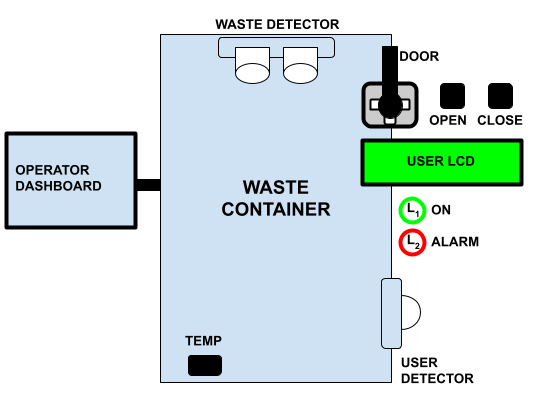
\includegraphics[width=240pt]{img/Assignment-02_SWDS-Domain.png}
        	\caption{Smart Waste Disposal System}
        	\label{img:system}
        \end{figure}
        \centerline{\href{https://docs.google.com/document/d/1iFXGmo7RVZMpJ5bxUN5ms_qFqg2B-wecRc0sfas9rQ4/edit?tab=t.0}{Here} is the complete description for the assignment.}
            
    \section{Domain Model}
    
        The waste container will manage an user detector. If an user is detected, in case the system was asleep it would be awaken, otherwise kept awake. If for some time no one is detected the system will turn in \textit{sleep mode} in order to consume less energy.
        %
        Moreover it will manage the door, which can be opened by the user pressing the ``Open'' button and can be closed by the user pressing the ``Close'' button otherwise after a timeout. The door will automatically close if sensors detect that the container is full or the temperature of the liquid too high. 
        Even the operator can open and close the door through his dashboard to empty the container. 
        %
        Furthermore it will manage the information devices: two leds and a display.
        The green one denote that there are no problems in the container and a user can spill his waste, while the red one indicates either the container is full or the liquid inside is too hot. 
        %
        The display will show a message to the user depending on the state of the container.\\\\
        %
        The operator dashboard let the operator to see the current data of the container's sensors, so the filling percentage and the temperature of the liquid inside. It offers also a button to empty the container, and a button to manage temperature problem inside the container. It can eventually show an history graph.\\\\
        %
        The waste container and the operator dashboard have to communicate. More specifically the dashboard will read from the waste container sensors data and will send a signal to empty or restore the container. 
            
    \section{Requirements}

        \subsection{Mandatory:}

            \begin{itemize}
                \item The system has to turn in \textit{sleep mode} if no user is detected for $T_
                {sleep}$ seconds. 
                \item The system has to wake up whenever an user is detected
                \item When the user presses the ``Open" button the container's door opens to let him spill waste.
                \item When the user presses the ``Close" button or $T_1$ seconds are elapsed from the opening of the container, the door will close. 
                \item The filling sensor is constantly checking for the filling level of the container, sending it to the operator dashboard. 
                \item Whenever the filling sensor detects that the container is full, it doesn't accept anymore waste until an operator empties it. If the door is open when the temperature exceeds his threshold it will immediately close. 
                \item The temperature sensor constantly checks the waste temperature sending it to the operator dashboard. 
                \item Whenever the temperature sensor detects a too high temperature in the liquid, the container doesn't accept anymore waste until the intervention of an operator. If the door is open when the temperature exceeds his threshold it will immediately close. 
                \item The display has to show different messages depending on the container's state. 
                \item When entering the spill is available it will be on the green led, while when is not available - in case of full container or waste with too high temperature - it will be on the red led.  
                \item The operator dashboard displays the current state of the container, in particular the filling percentage and the waste temperature. 
                \item An operator can empty the container through his dashboard pressing the button ``Empty the container". When the container has to empty the door will open for $T_3$ seconds. After emptying the container will be available for users. 
                \item In case of high temperature in the waste the operator can restore the container by pressing the ``Restore" button in the operator dashboard, making the container available for users.
            \end{itemize}

        \subsection{Optional:}
            
            \begin{itemize}
                \item The operator dashboard can store data to make an history graph.
            \end{itemize}

\chapter{Design}

    \section{Architecture}

        The system is composed by two modules: the container module and the operator module.
        The two modules can exchange information between each other by a serial line.\\\\
        %
        The container module is a task-based architecture. Tasks are concurrent and can interact one another by setting and reading shared flags. Tasks are executed by a cooperative scheduler.
        More specifically there are four tasks to manage the following behaviors: user management, filling percentage, waste temperature and communication with the operator dashboard.\\\\ 
        %
        The operator module is an active GUI showing the container's information and saving them to produce an history graph.
        It offers two buttons to manage issues of the container, namely the container full or the high temperature of the waste.

        \section{Detailed Design}

\chapter{Develop}

\appendix
\chapter{User Guide}

\end{document}